\section{Simulations}
\label{sec:simulations}

To assess the nature of the BAO signal in the DESI bispectrum we use \texttt{FirstGen} simulations. These simulations are based on \texttt{AbacusSummit} N-body simulations. The halos in the \texttt{AbacusSummit} have been populated with galaxies using the \textcolor{red}{we will describe how the FirstGens were produced here}. These HOD parameters were derived by fitting the projected small-scale clustering of the DESI Early Data Release sample. 

We use \texttt{Molino} simulations to assist in constructing covariance matrices. \texttt{Molino} simulations are based on the \texttt{Quijote} N-body simulation suit. They were constructed by \textcolor{red}{Same thing here}.

We use the \texttt{GLAM} simulations for constructing some of our BAO fitting templates. \textcolor{red}{we will describe the volume the number, etc}. Each instance of the \texttt{GLAM} simulations was run with a paired simulation with no input BAO signal. 

Molino (15,000 Mocks): 
$\Omega_{M}=0.32$, $\sigma_{8}=0.834$, Volume $\sim 1 {\rm Gpc}/h^{3}$ 
Galaxy catalogs from the Quijote N-body simulations (Villaescusa-Navarro et al.2020) with the standard Halo Occupation Distribution model from Zheng et al. (2007). HOD parameters are based on high luminosity SDSS samples. More at changhoonhahn.github.io/molino

And two other series of mocks provided by our DESI collaborators:
GLAM (1,000 Mocks)

Abacus (25 mocks)


Fig. \ref{fig:data} shows the mean bispectrum (left) and the mean power spectrum (right) for the GLAM and ABACUS simulations, relative to the spectra without the BAO signal, which is simulation-based for the GLAM realizations and theory-based for the ABACUS.

\begin{figure*}
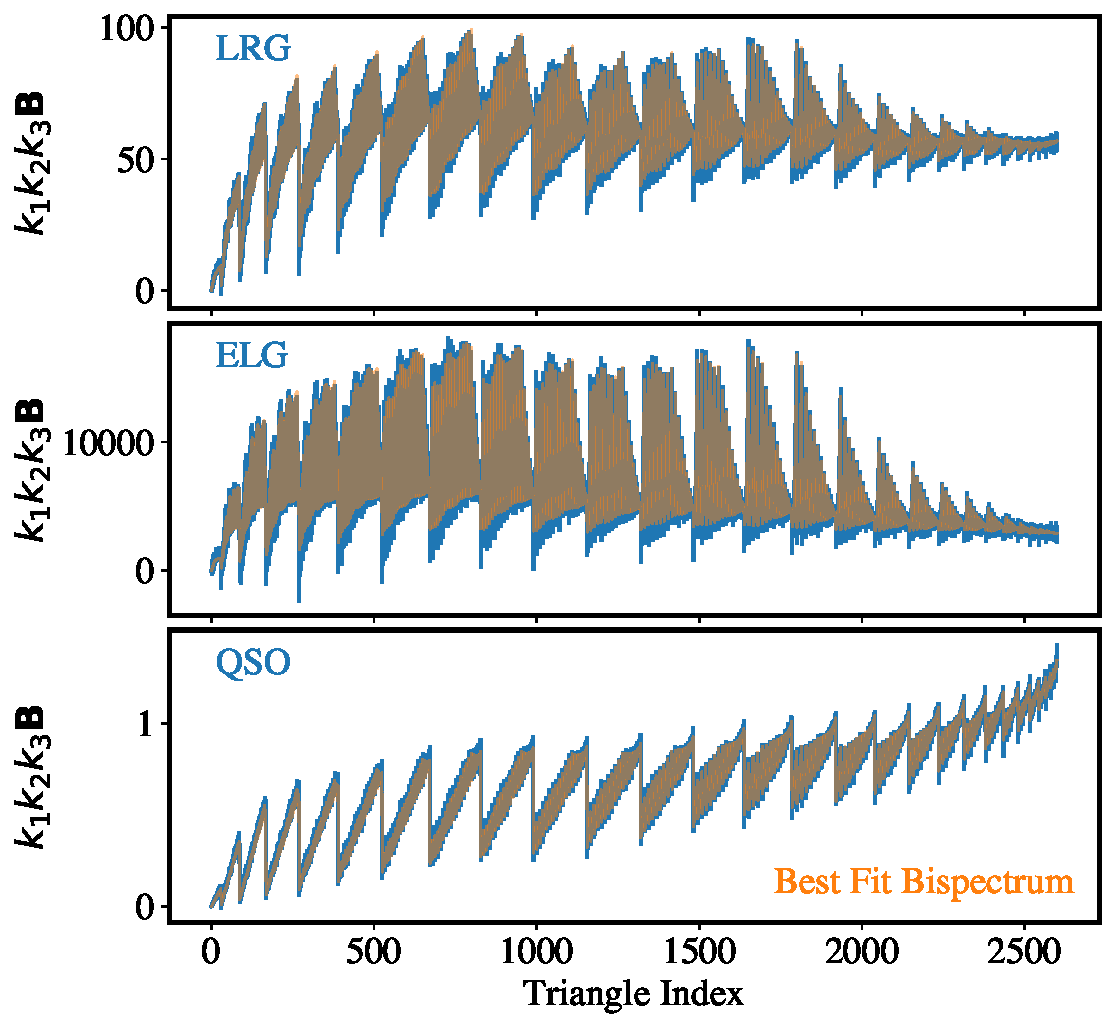
\includegraphics[width=\textwidth]{figures/spectra.pdf}
\caption{Spectra of ABACUS, GLAM, and MOLINO simulations. Top: Mean bispectrum and power spectrum of simulations relative to smooth spectrum either from the mocks (GLAM) or fitting formula (ABACUS). Bottom: Normalized dispersion of bispectrum and power spectrum.}\label{fig:data}
\end{figure*}


We estimate the reduced covariance matrix from a suite of 15000 simulations (MOLINO) and scale it by the variance of power spectrum or bispectrum for the GLAM or ABACUS realizations.